
         %% %% %% %%         Preamble & Options          %% %% %% %%
%~~~~~~~~~~~~~~~~~~~~~~~~~~~~~~~~~~~~~~~~~~~~~~~~~~~~~~~~~~~~~~~~~~~~~~~~~~~~~~%
\documentclass[paper=a4,fontsize=10pt,DIV=18,twocolumn,parskip=half]{scrartcl}
%%%%%%%%%%%%                      PACKAGES                           %%%%%%%%%%%
%~~~~~~~~~~~~~~~~~~~~~~~~~~~~~~~~~~~~~~~~~~~~~~~~~~~~~~~~~~~~~~~~~~~~~~~~~~~~~~%
\usepackage[utf8]{inputenc}		% utf8 encoding für umlaute und sonderzeichen
\usepackage[ngerman,english]{babel} 	% hyphenations in  different languages
\usepackage[tbtags]{amsmath}    % tbtags sets the number of split 
                                % environments at the end 
\usepackage{amssymb} 	    	% symbols
\usepackage{amsfonts} 	    	% font
\usepackage{textcomp} 		    % degree signs -> \textdegree
\usepackage{siunitx}		    % correct units and spacing
\usepackage{hyperref}	        % references and links
\usepackage{graphicx}           % embedd images
\usepackage{tikz}			    % tikz painting, e.g circled text
\usepackage{subfig}				% subfigure for mutliple pictures
\usepackage{color}              % define own colors
\usepackage[font=small,labelfont=bf,format=plain,margin=10pt]{caption}
\usepackage[noabbrev]{cleveref}
\usepackage{bijan_commands}     % self defined commands and shorthand notations
                                % !! has to be added manually !!


%\usepackage{pdfsync}		    % pdf synchronization (reverse search)
%\usepackage{booktabs}	        % nice table lines
%\usepackage{fancyhdr} 			% headers and footers
%\usepackage{fancybox} 			% boxes with rounded corners 
%\usepackage{wrapfig} 		    % figures floating beside the text
%\usepackage{picinpar}			% textbox beside the text
%\usepackage{placeins}			% float barriers in sections
%\usepackage{moreverb}
%\usepackage{listings}
%\usepackage{pifont} 			% DING fonts (used in the acknowledgement)
%\usepackage{scrtime}           % current time 
%\usepackage[numbers,sort&compress]{natbib} 		
                                % sorted references  with clickable URL 
%\usepackage{makeidx} 			% index at the end
%\usepackage[chapter,numbib]{tocbibind}     % add several things to the TOC


%%%%%%%%%%%                        SETUP                             %%%%%%%%%%%
%~~~~~~~~~~~~~~~~~~~~~~~~~~~~~~~~~~~~~~~~~~~~~~~~~~~~~~~~~~~~~~~~~~~~~~~~~~~~~~%
% color:
\definecolor{darkblue}{rgb}{0,0,0.5}
\definecolor{lila}{rgb}{0.3,0,0.3}
\definecolor{turq}{rgb}{0,0.1,0.4}

% siunitx:
\sisetup	{separate-uncertainty, per-mode=fraction}

% hyperref:
\hypersetup{	pdftex,
                colorlinks=true,
                backref=page,
                linkcolor=darkblue,     % usual links
                filecolor=red,
                citecolor=turq,  	    % for bibliographic
                urlcolor=lila,  		% for Emails and URLs
                pdfpagelabels=true, 	% that the pagenumbering is ok 
                breaklinks=true,
                plainpages=false,
                bookmarks=true, 
                bookmarksnumbered=false
                %pdftitle={--title--},
                %pdfauthor={--author--},
                %pdfsubject={},
                %pdfkeywords={--kind-of-work--},
            }

% hyperref:
% set black for printing	
% \hypersetup{
    % colorlinks,
    % citecolor=black,
    % filecolor=black,
    % linkcolor=black,
    % urlcolor=black
    % }

%tocibind:
%\setcounter{tocdepth}{2} % change to 1 that not so deep (smaller TOC)
           % defines packages and setups
%~~~~~~~~~~~~~~~~~~~~~~~~~~~~~~~~~~~~~~~~~~~~~~~~~~~~~~~~~~~~~~~~~~~~~~~~~~~~~~%
\numberwithin{equation}{section}    % number equations after sections
\columnsep20pt                      % width between \twocolumns
\linespread{1.2}
\allowdisplaybreaks[1]              % permissiveness of page breaks in equations
                                    % 1 ="allow page breaks but avoid them" 
                                    % and 4="break whenever you want".

%%% Spacings:
\setlength{\headheight}{2.0\baselineskip}       
% Fixes the 'small headhight'

\renewcommand*{\chapterheadstartvskip}{\vspace{0\baselineskip}} 
% Spacing Pagehead-Headline. Standard: 2

\renewcommand*{\chapterheadendvskip}{\vspace{\baselineskip}}
% Spacing Headline-Text

%%%%%%%%% %%%%%%%%% %%%%%%%%% %%%%%%%%% %%%%%%%%% %%%%%%%%% %%%%%%%%% %%%%%%%%%%


\begin{document}

\title{Projekt zum Fortgeschrittenen-Praktikum \\ - Atomic Force Microscopy}                  
\author{Guilherme Stein \& Ulrich Müller}         
\date{}                             % Turn off automatic date
\twocolumn[\begin{@twocolumnfalse}
\vspace{-3em}
\maketitle      
% =============================================================================
\begin{abstract}      
% =============================================================================
  \vspace{-2em}
  \noindent {\small 
  % abstact 
    }
  \vspace{1em}

  \noindent Supervisor: Dr. Paolo Sessi
  \hfill Date of experiment: $4^{\text{th}}$ October 2013
  \begin{flushright}
    % Protokollabgabe: 12. Oktober 2012        
  \end{flushright}
\end{abstract}
\vspace{2em}
%
\end{@twocolumnfalse}
]
% =============================================================================
%\addtocounter{section}{-1}
\section{Expose}
The III-V semiconductor system based on GaSb is commonly used for optical semiconductor devices with wavelengths beyond $\SI{2.3}{\micro\meter}$ \cite{arafin}. In Würzburg especially the interband cascade lasers, which are grown by MBE on GaSb substrate, made significant progress during the last years \cite{weih}. In order to grow devices with high performance it is inevitable to use high quality substrates with a minimum of defects. Despite the use of epi-ready substrates the wafers suffer from native oxide like $\mathrm{Ga}_2 \mathrm{O}_3$ and $\mathrm{Sb}_2 \mathrm{O}_3$ \cite{vineis}. The growth of devices on top of this oxide would lead to non-monocrystal layers. To remove this oxide a commonly used technique in Würzburg is to heat the substrate to about $\SI{580}{\degree}$ for short time. At this temperature the most of the oxide desorbes from the surface  but leaving holes in the surface with the size in the order of  $\SI{10}{\nano\meter}$ \cite{murray}. Hereupon a $\SI{200}{\nano\meter}$ GaSb buffer layer is grown at $\SI{485}{\degree}$ to flatten the surface. This method has been established during the last years although it has never been investigated whether a different technique would lead to smoother surfaces. 
To characterize the smoothness of a surface one needs a proper definition of this physical property:\\
	unsere Definition\\
A Atomic Force Microscope (AFM) is the perfect instrument to characterize this smoothness of the wafers. \\
	AFM Beschreibung\\
As the AFM doesn't work in situ we have to produce and investigate the surface at each step of the growth process to understand the mechanisms of oxide desorbtion and flattening of the surface. We going to characterize the single steps of the standard process which are: an untreated GaSb Wafer, the Wafer after the oxide desortion and after $\SI{200}{\nano\meter}$ GaSb buffer. To vary this process we want to test two aspects: first the increase of the GaSb buffer's growth temperature up to $\SI{500}{\degree}$ and $\SI{515}{\degree}$ and second the growth of a $\SI{30}{\nano\meter}$ GaSb/AlAsSb superlattice directly after oxide desorbtion. Recent research showed that the growth of AlAsSb shutting down the step-flow growth mode which is dominant in the growth of GaSb layers and is not very successful in flattening bigger defects like defects in pyramidal shape. The growth of a superlattice is nevertheless necessary to maintain the electrical conductivity of the sample.\\
It would be helpful to understand how these defects are removed from the surface and how the process can be improved as theses pyramidal defects tend to grow bigger as the growth progresses. After the growth of structures with a thickness of several microns these defects can even be observed by a optical microscope with a magnification of $50$.
\begin{figure}[htb]
  \includegraphics[width=\linewidth]{Bilder/A2749_50_1}
  \caption{At the samples' surface after several micrometer growth small pyramidal defects are visible. The image was taken by an optical microscope at a magnification of 50.}
  \label{bandluecke}
\end{figure}



%Materialsystem GaSb
%Optische Elemente/Laser
%Wachstum ohne Defekte wünschenswert
%native Oxid on epi-ready wafer.
%Standardverfahren beschreiben
%	Oxiddesorption
%	Bufferwachstum
%Wollen Verfahren variieren und  mit AFM zeigen, wie sich die Oberflächenrauigkeit verändert.
%AFM-Einleitung
%	Entdeckung
%	Funktion
%	etc...
%Proben
%1. nur Oxiddesorption
%2. Standard
%4. höhere Wachstumstemperaturen
%5. noch höhere Wachstumstemperaturen
%7. mit AlAsSb Übergitter 
%8. höhere Wachstumstemperaturen und AlAsSb 			    Übergitter 
%	oder 300nm Buffer
%	oder längere Oxiddesorption
%
%	
%Rauigkeit definieren
%	Über Blöcke der Größe Lambda mitteln; Dann Oberflächenspannung
%Mikroskopbilder hinzufügen
%
%Zitate


\label{Expose}
\newpage

\section{Basics}
%Warum AFM\\
The relevance of fabrication and therefore also the analysis of structure in the 
sub-micrometer and even nanometer scale has increased steadily in the past 
decades. In contrast to other scanning imaging techniques as the STM or SEM, the 
atomic force microscope (AFM) is capable to deliver up to atomic resolution 
without the need of a vacuum or special treatment of the probe prior to 
analysis. This allows us to examine a broader variety of samples under easily 
achievable conditions.

\subsection{Work principle of the AFM}
%Funktionsweise AFM\\
The principle of the atomic force microscope are the forces that act between two 
pieces of matter when brought close to each other. More precisely we bring a 
sharp tip into a distance of a few nano meters to  a surface we want to examine.  
scale the main contribution are Van-der-Waals forces which arise from 
polarisation fluctuations in the material.
In \cref{afm_scheme} one can see the main parts required to run the AFM. 
The sample is mounted on a xyz-stage consisting of different piezo elements. 
This enables us to move the sample in xy-direction for the scanning of the 
probe, as well as in the z direction for height compensation. A reflecting 
cantilever is positioned above the sample. A laser beam will reflect on the 
cantilever and hits a segmented photodiode. If the cantilever moves, the 
laser beam will change the angle of deflection, detectable by the photodiode.
From the intensity change on the diode segments one can calculate the height 
difference of the material.

\begin{figure}
    \centering
    \includegraphics{Bilder/afm_scheme.pdf}
    \caption{Simplified illustration of an atomic force microscope}
    \label{afm_scheme}
\end{figure}

\subsection{Refinements}
Instead of mapping the intensity change on the diode to the force and 
subsequently to the probe height, often a different approach is used. The tip is 
set to apply a constant force on the probe. If the force changes, the piezo in 
z-direction is altered to move the probe to a height where the force is equal to 
the set point defined before. This has the advantage that the force between tip 
and probe is approximately constant and therefore it is less likely to damage 
the sample or the tip. This is ensured via a feedback loop between the the diode 
and the piezo element as seen in \cref{control_loop}.

\begin{figure}
    \centering
    
\includegraphics{Bilder/control_loop.pdf}
    \caption{Principle of a feedback loop with disturbance $z(t)$, output 
        $r(t)$, control signal $u(t)$, measured output $x(t)$ and error signal 
        $e(t)$.}
    \label{control_loop}
\end{figure}

The height information accquired via this method is more strongly connected to 
the actual sample surface. The mapping is done between the piezo voltage as 
opposed to the strength of the diode, the angle of the lase beam and the 
distances between those elements. Therefore introducing less error sources and 
leading to a more accurate signal.

%
Relevanz für die Aufnahme der GaSb Proben\\
%

\section{Data Aquisition}
\label{dataaquisition}
In order to acquire the topology of the samples surface the computer records the 
z-position in combination with the x- and y-position of the Auswirkungen der 
PI-Parameter\\
To optimize the quality of the pictures we can adjust the P- and I-values. These 
values refer to the proportional and integral-gain of the z-controllers feedback 
loop respectively. To 

For a topographical imaging mode, a feedback loop (Fig. 4.3) is implemented to 
keep the cantilever deflection constant by changing the tip height (z) while 
scanning in x and y. In this way, a nearly constant force is maintained between 
the tip and sample, and the topographical image is created by recording the 
voltage applied to the z-piezo as a function of the x and y position. As the tip 
is scanned,  lateral force are


Format\\
Rauschen- SNR  Arten \\
Methoden und Probleme der Bildbearbeitung\\
\section{Sample Analysis}
Features\\
Rauigkeit der Oberfläche\\
Aussagen über Wachstumsmethoden\\


% =============================================================================
\begin{thebibliography}{}   
% =============================================================================

\bibitem{arafin} Shamsul Arafin (2012): Electrically-Pumped GaSb-Based 
Vertical-Cavity Surface-Emitting Lasers. München.

\bibitem{weih} Weih, Robert; Kamp, Martin; Höfling, Sven (2013): Interband 
cascade lasers with room temperature threshold current densities below 100 
A/cm2. In: Appl. Phys. Lett. 102 (23), S. 231123. DOI: 10.1063/1.4811133.

\bibitem{vineis} C.J. Vineis; C.A. Wang; K.F. Jensen (2001): In-situ reflectance 
monitoring of GaSb substrate oxide desorption 2001.

\bibitem{murray} Murray, Lee M.; Yildirim, Asli; Provence, Sydney R.; Norton, 
Dennis T.; Boggess, Thomas F.; Prineas, John P. (2013): Causes and elimination 
of pyramidal defects in GaSb-based epitaxial layers. In: J. Vac. Sci. Technol. B 
31 (3), S. 03C108. DOI: 10.1116/1.4792515.
  

\end{thebibliography}
%
%
\onecolumn
\pagestyle{empty}
%% =============================================================================
%\section{Anhang}
%\label{Anhang}
%% =============================================================================

\end{document}



%% =============================================================================
%%%%%%%%%%%%%%%%%%% OBSOLETE (can be removed) %%%%%%%%%%%%%%%%%%%%%%%%%%
%% =============================================================================

%\usepackage[font=small,labelfont=bf,format=plain,margin=10pt]{caption}
%\usepackage{bijan_koma}
%\usepackage[ngerman]{babel} 

%%%%%%%%%%%%%%%%%%%%%% Settings for packages %%%%%%%%%%%%%%%%%%%%%%%%%%%%%%%%%%

%\usepackage[range-phrase={\,\,bis\,\,}]{siunitx}  % Correct typesetting of units
%\sisetup{       
  %separate-uncertainty,
  %per-mode=fraction
%}

%\colorlet{darkblue}{blue!70!black}
%\hypersetup{
  %colorlinks,
  %citecolor=darkblue,
  %filecolor=darkblue,
  %linkcolor=darkblue,
  %urlcolor=black
%}

%\crefformat{equation}{Glg.~(#2#1#3)}
%\crefformat{section}{Abschnitt~#2#1#3}
%\crefformat{figure}{Abb.~#2#1#3}
%\crefformat{table}{Tab.~#2#1#3}
%\crefformat{chapter}{Kapitel~#2#1#3}


%\addto\captionsngerman{             % Changes Abbildung->Abb.,etc. in caption 
  %\renewcommand{\figurename}{Abb.}
  %\renewcommand{\tablename}{Tab.}
%}


%%%%%%%%%%%%%%%%%%%%%% Headings and seperation lines %%%%%%%%%%%%%%%%%%%%%%%%%%


%\usepackage[automark,markuppercase]{scrpage2}     % AUTOMATIC HEADINGS
%\pagestyle{scrheadings}                           % Apply userdefined settings
%\setheadsepline{.5 pt}                            % Width of seperation line
%\setkomafont{pagehead}{\normalfont}               % Use normalfont for heading
%\cfoot{\thepage}                                  % Page numbering 

%%%%%%%%%%%%%%%%%%%%%% commands      %%%%%%%%%%%%%%%%%%%%%%%%%%
%\newcommand*\circled[1]{\tikz[baseline=(char.base)]{
            \node[shape=circle,draw,inner sep=0.4pt] (char) {#1};}} 	%circled text with tikz
			
\newcommand{\tabref}[1]{Table~\ref{tab:#1}}
\newcommand{\figref}[1]{Figure~\ref{fig:#1}}
\newcommand{\secref}[1]{section~\ref{sec:#1}}
\renewcommand{\eqref}[1]{(\ref{eq:#1})}
\newcommand{\ket}[1]{\left| #1 \right>}
\newcommand{\bra}[1]{\left< #1 \right|}
\newcommand{\braket}[2]{\left< #1 \vphantom{#2}  \, \right| \left. \vphantom{#1} #2 \right>}
\newcommand{\uuline}[1]{\underline{\underline{#1}}}				% double underline
\newcommand{\vop}[1]{\ensuremath{\mathbf{\hat{#1}}}} 		% vector operator
\newcommand{\vect}[1]{\ensuremath{\boldsymbol{#1}}} 			% bold vector
\newcommand{\abs}[1]{\lvert#1\rvert}										% absolute
\newcommand{\norm}[1]{\lVert#1\rVert}									% norm

%\newcommand{\tabref}[1]{Table~\ref{tab:#1}}
%\newcommand{\figref}[1]{Figure~\ref{fig:#1}}
%\newcommand{\secref}[1]{section~\ref{sec:#1}}

%\graphicspath{{Bilder/}}
%%%%%%%%%%%%%%%%%%%%%% Spacings %%%%%%%%%%%%%%%%%%%%%%%%%%%%%%%%%%%%%%%%%%%%%%%

%\onehalfspacing                                 % 1.5 line spacing

% Spacing in math environments \,\;.. 
%\thinmuskip=3mu % default
%\medmuskip=4mu plus 2mu minus 4mu % default is 4 mu p2 m4
%\thickmuskip=5mu plus 5mu % default


